\documentclass[tikz,border=12pt]{standalone}
\usepackage[T1]{fontenc}
\usepackage{mathpazo}
\usepackage{amsmath,amssymb}
\usetikzlibrary{arrows.meta, positioning, calc, fit, patterns, decorations.pathreplacing}

\definecolor{stblue}{HTML}{7B97AD}
\definecolor{rwgold}{HTML}{B8995E}
\definecolor{sage}{HTML}{7A9A7E}
\definecolor{dkbrown}{HTML}{3D3530}
\definecolor{wmgray}{HTML}{7B7067}
\definecolor{cream}{HTML}{F9F6F0}
\definecolor{border}{HTML}{D4C9B8}
\definecolor{terracotta}{HTML}{C47A6A}
\definecolor{lavender}{HTML}{907EA0}

\begin{document}
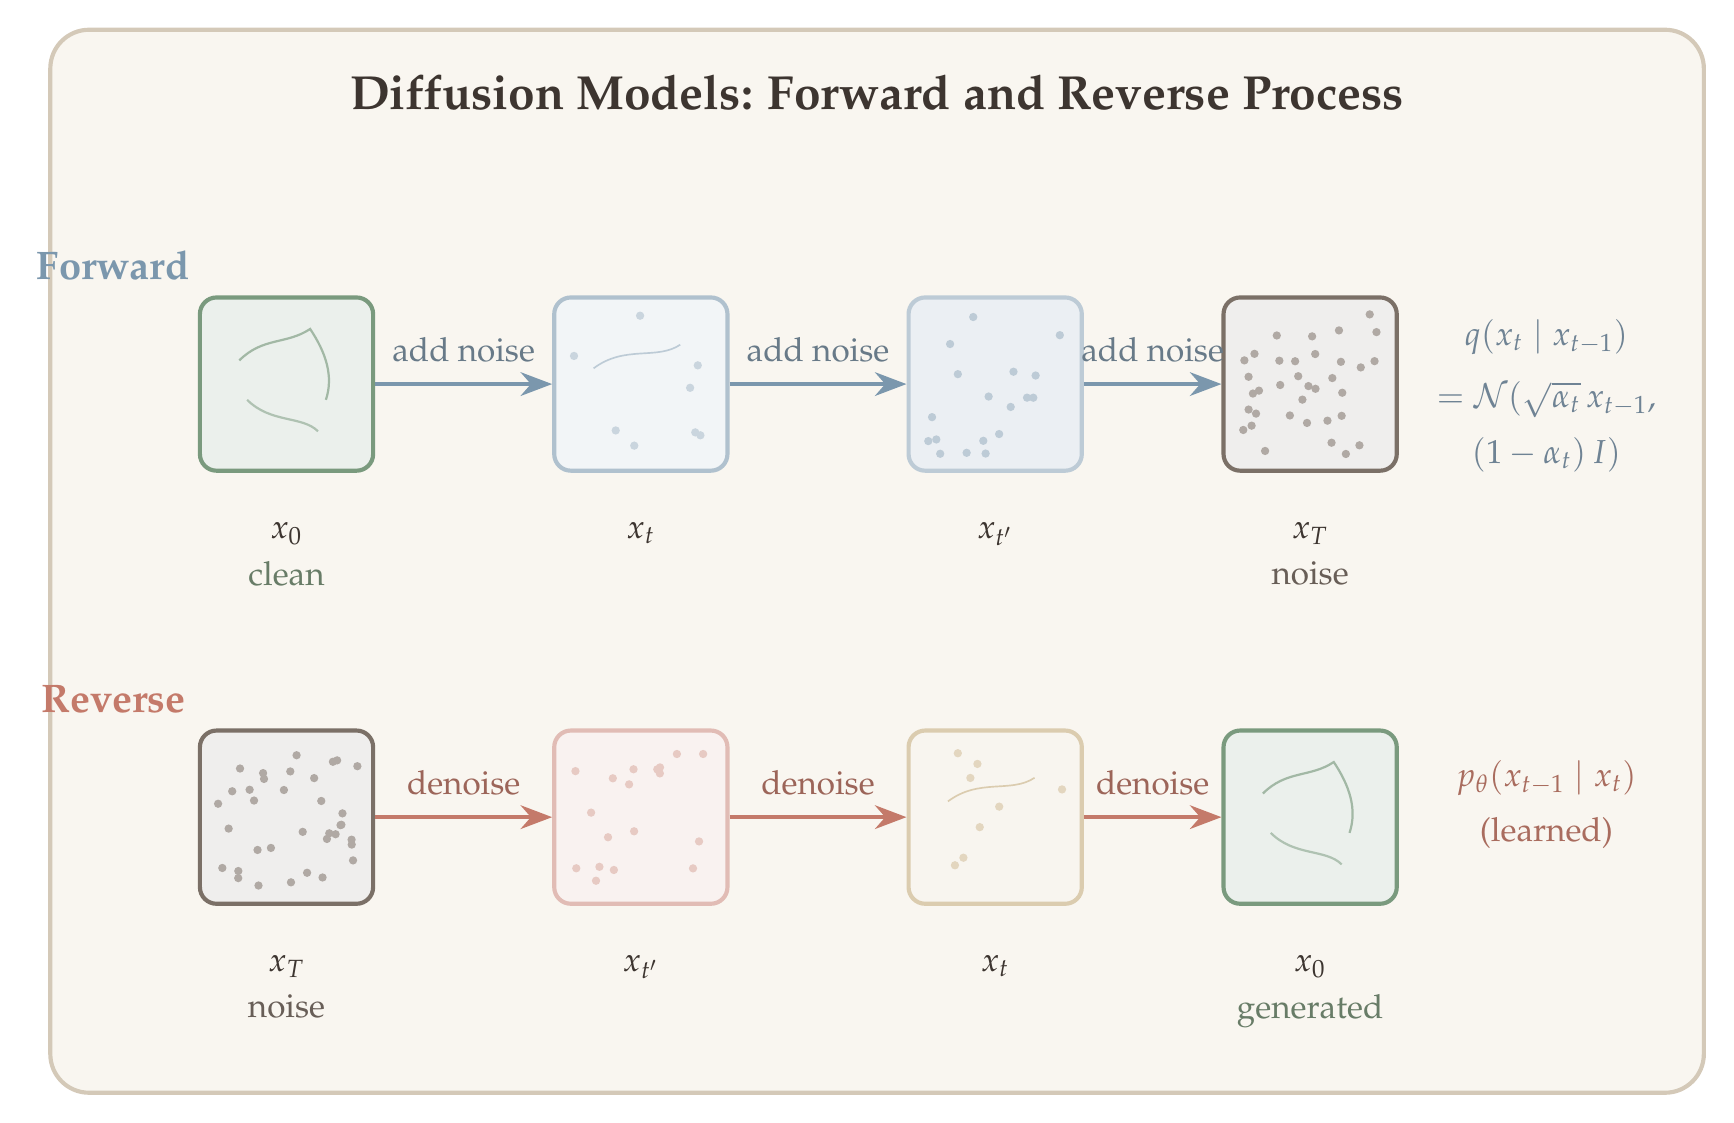
\begin{tikzpicture}[>={Stealth[length=4mm, width=3mm]}, line width=1.5pt]

% Background
\fill[cream, rounded corners=14pt] (-1,-7) rectangle (20,6.5);
\draw[border, line width=1.5pt, rounded corners=14pt] (-1,-7) rectangle (20,6.5);

% Title
\node[font=\LARGE\bfseries, text=dkbrown] at (9.5,5.7) {Diffusion Models: Forward and Reverse Process};

% ========== Forward process (top row) ==========
\node[font=\Large\bfseries, text=stblue] at (-0.2,3.5) {Forward};

% Stage boxes - progressively noisier
% Clean data x_0
\node[fill=sage!15, draw=sage, line width=1.5pt, rounded corners=6pt,
      minimum width=2.2cm, minimum height=2.2cm] (f0) at (2,2) {};
\draw[sage!70, line width=0.8pt] (1.4,2.3) .. controls (1.7,2.6) and (2.0,2.5) .. (2.3,2.7)
  .. controls (2.5,2.4) and (2.6,2.1) .. (2.5,1.8);
\draw[sage!60, line width=0.8pt] (1.5,1.8) .. controls (1.8,1.5) and (2.2,1.6) .. (2.4,1.4);
\node[font=\large, text=dkbrown, below=14pt] at (f0.south) {$x_0$};
\node[font=\large, text=sage!70!dkbrown, below=28pt] at (f0.south) {clean};

% x_{t/3}
\node[fill=stblue!10, draw=stblue!60, line width=1.5pt, rounded corners=6pt,
      minimum width=2.2cm, minimum height=2.2cm] (f1) at (6.5,2) {};
\foreach \i in {1,...,8} {
  \pgfmathsetmacro{\rx}{5.6 + rnd*1.8}
  \pgfmathsetmacro{\ry}{1.1 + rnd*1.8}
  \fill[stblue!40] (\rx,\ry) circle (1.5pt);
}
\draw[stblue!50, line width=0.6pt] (5.9,2.2) .. controls (6.3,2.5) and (6.7,2.3) .. (7.0,2.5);
\node[font=\large, text=dkbrown, below=14pt] at (f1.south) {$x_t$};

% x_{2t/3}
\node[fill=stblue!15, draw=stblue!50, line width=1.5pt, rounded corners=6pt,
      minimum width=2.2cm, minimum height=2.2cm] (f2) at (11,2) {};
\foreach \i in {1,...,18} {
  \pgfmathsetmacro{\rx}{10.1 + rnd*1.8}
  \pgfmathsetmacro{\ry}{1.1 + rnd*1.8}
  \fill[stblue!50] (\rx,\ry) circle (1.5pt);
}
\node[font=\large, text=dkbrown, below=14pt] at (f2.south) {$x_{t'}$};

% Pure noise x_T
\node[fill=wmgray!12, draw=wmgray, line width=1.5pt, rounded corners=6pt,
      minimum width=2.2cm, minimum height=2.2cm] (f3) at (15,2) {};
\foreach \i in {1,...,35} {
  \pgfmathsetmacro{\rx}{14.1 + rnd*1.8}
  \pgfmathsetmacro{\ry}{1.1 + rnd*1.8}
  \fill[wmgray!60] (\rx,\ry) circle (1.5pt);
}
\node[font=\large, text=dkbrown, below=14pt] at (f3.south) {$x_T$};
\node[font=\large, text=wmgray!70!dkbrown, below=28pt] at (f3.south) {noise};

% Forward arrows
\draw[->, stblue, line width=1.5pt] (f0.east) -- (f1.west)
  node[midway, above=4pt, font=\large, text=stblue!70!dkbrown] {add noise};
\draw[->, stblue, line width=1.5pt] (f1.east) -- (f2.west)
  node[midway, above=4pt, font=\large, text=stblue!70!dkbrown] {add noise};
\draw[->, stblue, line width=1.5pt] (f2.east) -- (f3.west)
  node[midway, above=4pt, font=\large, text=stblue!70!dkbrown] {add noise};

% Forward process label
\node[font=\large, text=stblue!80!dkbrown] at (18,2.6) {$q(x_t \mid x_{t-1})$};
\node[font=\large, text=stblue!80!dkbrown] at (18,1.8) {$= \mathcal{N}(\sqrt{\alpha_t}\, x_{t-1},$};
\node[font=\large, text=stblue!80!dkbrown] at (18,1.1) {$(1-\alpha_t)\, I)$};

% ========== Reverse process (bottom row) ==========
\node[font=\Large\bfseries, text=terracotta] at (-0.2,-2) {Reverse};

% Pure noise
\node[fill=wmgray!12, draw=wmgray, line width=1.5pt, rounded corners=6pt,
      minimum width=2.2cm, minimum height=2.2cm] (r3) at (2,-3.5) {};
\foreach \i in {1,...,35} {
  \pgfmathsetmacro{\rx}{1.1 + rnd*1.8}
  \pgfmathsetmacro{\ry}{-4.4 + rnd*1.8}
  \fill[wmgray!60] (\rx,\ry) circle (1.5pt);
}
\node[font=\large, text=dkbrown, below=14pt] at (r3.south) {$x_T$};
\node[font=\large, text=wmgray!70!dkbrown, below=28pt] at (r3.south) {noise};

% Partially denoised
\node[fill=terracotta!10, draw=terracotta!50, line width=1.5pt, rounded corners=6pt,
      minimum width=2.2cm, minimum height=2.2cm] (r2) at (6.5,-3.5) {};
\foreach \i in {1,...,18} {
  \pgfmathsetmacro{\rx}{5.6 + rnd*1.8}
  \pgfmathsetmacro{\ry}{-4.4 + rnd*1.8}
  \fill[terracotta!40] (\rx,\ry) circle (1.5pt);
}
\node[font=\large, text=dkbrown, below=14pt] at (r2.south) {$x_{t'}$};

% More denoised
\node[fill=rwgold!10, draw=rwgold!50, line width=1.5pt, rounded corners=6pt,
      minimum width=2.2cm, minimum height=2.2cm] (r1) at (11,-3.5) {};
\foreach \i in {1,...,8} {
  \pgfmathsetmacro{\rx}{10.1 + rnd*1.8}
  \pgfmathsetmacro{\ry}{-4.4 + rnd*1.8}
  \fill[rwgold!40] (\rx,\ry) circle (1.5pt);
}
\draw[rwgold!50, line width=0.6pt] (10.4,-3.3) .. controls (10.8,-3.0) and (11.2,-3.2) .. (11.5,-3.0);
\node[font=\large, text=dkbrown, below=14pt] at (r1.south) {$x_t$};

% Generated image
\node[fill=sage!15, draw=sage, line width=1.5pt, rounded corners=6pt,
      minimum width=2.2cm, minimum height=2.2cm] (r0) at (15,-3.5) {};
\draw[sage!70, line width=0.8pt] (14.4,-3.2) .. controls (14.7,-2.9) and (15.0,-3.0) .. (15.3,-2.8)
  .. controls (15.5,-3.1) and (15.6,-3.4) .. (15.5,-3.7);
\draw[sage!60, line width=0.8pt] (14.5,-3.7) .. controls (14.8,-4.0) and (15.2,-3.9) .. (15.4,-4.1);
\node[font=\large, text=dkbrown, below=14pt] at (r0.south) {$x_0$};
\node[font=\large, text=sage!70!dkbrown, below=28pt] at (r0.south) {generated};

% Reverse arrows
\draw[->, terracotta, line width=1.5pt] (r3.east) -- (r2.west)
  node[midway, above=4pt, font=\large, text=terracotta!70!dkbrown] {denoise};
\draw[->, terracotta, line width=1.5pt] (r2.east) -- (r1.west)
  node[midway, above=4pt, font=\large, text=terracotta!70!dkbrown] {denoise};
\draw[->, terracotta, line width=1.5pt] (r1.east) -- (r0.west)
  node[midway, above=4pt, font=\large, text=terracotta!70!dkbrown] {denoise};

% Reverse process label
\node[font=\large, text=terracotta!80!dkbrown] at (18,-3.0) {$p_\theta(x_{t-1} \mid x_t)$};
\node[font=\large, text=terracotta!80!dkbrown] at (18,-3.7) {(learned)};

\end{tikzpicture}
\end{document}
